\subsection{The free Electron Model} \label{chap1}

By using the free electron model, some of the parameter
of a given metal can be calculated. The given metal
crystllizes in the fcc structure with a lattice parameter 
for the convential unit cell of $0.409nm$. And a given 
resistivity for room temperature.

(Source \cite[Elementary Solid State Physics Chapter 4]{elementary_SSP})

\subsubsection*{Collision Time}

For calculating the collision time the following relation
is used.

\begin{equation}
    \sigma = \frac{N e^2 \tau}{m^*}
\end{equation}


At it is a monovalent metal and the FCC-Unit cell contains 
4 atoms the concentration of the conduction electrons $N$ can be
calculated as ($a = 4.09 \mathring{A}$):

$$N =\frac{4}{a^3}$$

So for the collision time $\tau$ follows:
With $(m^* = m_0)$ the free electron mass.

The electrical resitivity is given as:
$\rho = 2.13 \mu \Omega cm$

which leads to a conducitivity of
$\sigma = \frac{1}{\rho} = 4.695\cdot 10^7 \frac{1}{\Omega m}$


$$\tau =\frac{\sigma \cdot m^* \cdot a^3}{4e^2} = 28.5 \cdot 10^{-14}s$$

\subsubsection*{Drift Velocitiy}

For a thin metal wire with a length of $10 \, cm$, a square cross section with 
a side of $0.1 \, mm$ and a potential difference along the wire of $0.2 \, V$

The electric field $E$ in the wire can be calculated as: 

$$E = \frac{U}{L} = 2 \frac{V}{m}$$

As for the current density the following relations are known.

$$J = \sigma E \qquad J = Nev_D$$

So for the drift velocitiy follows:

$$v_D =  \frac{\sigma E}{N e} = 1.003 \frac{m}{s}$$

\subsubsection*{Electron Disperion Phenomena and Resistitviy as function of Temperature}

In the free-electron model, the electron dispersion relation is,

$$E(\vec{k}) = \frac{\hbar^2k^2}{2m^*}$$

Here $m^*$ is the effective mass. At low temperature, all of
the $k$ states below the Fermi wave vector $k_F$ are filled 
and all the states above $k_F$ are empty (see the next subsection).

\autoref{fig:ek_allowed} a shows the electron diesperision in dependence o $k$.


The resitivity of a metal as a function of temperature can be best 
described by the following curve of Na.

\begin{figure}[H]
    \centering
    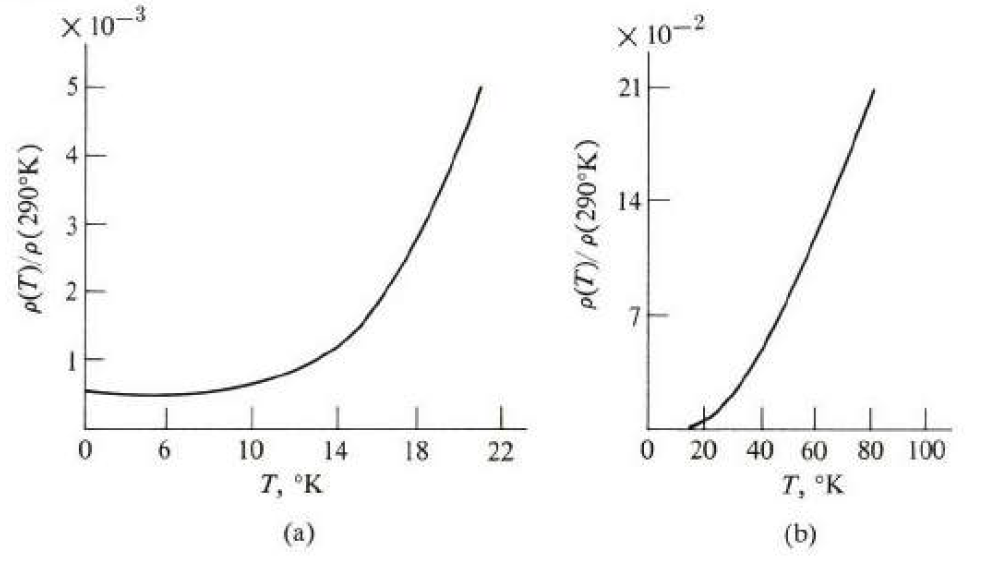
\includegraphics[width=0.6\linewidth]{Graphics/Chapter1/temp_resistitviy.png}
    \caption{The normailized resitivity $\rho(T)/\rho(290\degree K)$ versus $T$ 
    for Na in the low-temperature region (a), and at higher temperatures (b) 
    \cite[Elementary Solid State Physics p. 148]{elementary_SSP} }
    \label{fig:temp_resistitviy}
\end{figure}

At temperatures near $0 \degree K$ the resitivity has a small constant 
value. The resitivity increases with T \autoref{fig:temp_resistitviy} a.
For higher values for $T$ the value of the resistivity
increases linear with $T$. Room temperature $T=300\degree K$
usually falls in the linear region.

\subsubsection*{Fermi Energy and Fermi Surface}

The energy of the electron in a metal is quantized according to quantum mechanics.
As so they follow the \textit{Pauli exclusion principle}, which means only two 
electrons with different spin can occupy one energy level.
The highest occupied energy level is then called the Fermi energy or the fermy
level.

The situation described obtains in metals as $T=0 \degree K$. The probability that 
an level below the fermi energy is occupied is 1 and above equals 0.

If the system is heated, the electrons near the fermi level get excited as 
the electrons below the fermi level can not absorb energy due to the exclusion
principle.

Which leads to the \textit{Fermi-Dirac distribution}, which gives
the probability that the level $E$ is occupied by an electron

\begin{equation}
    f(E) = \frac{1}{e^{(E-E_F)/kT}+1}
\end{equation}

\begin{figure}[H]
    \centering
    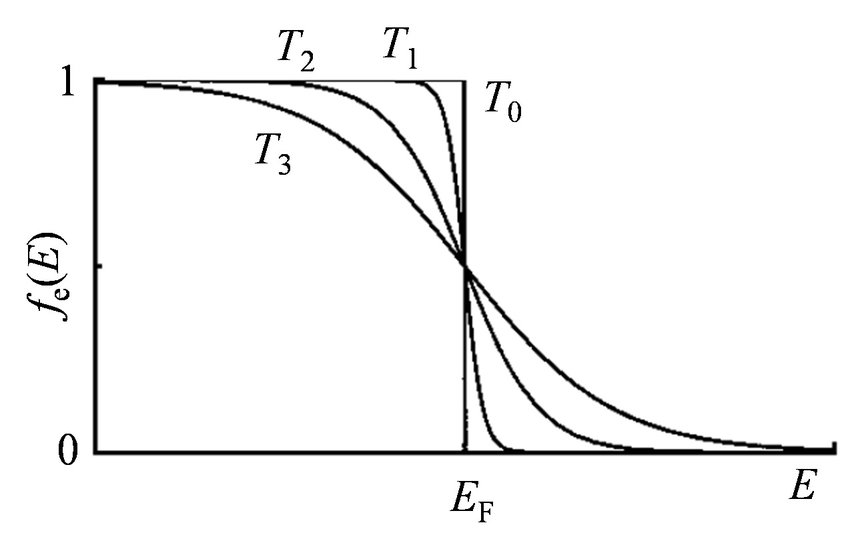
\includegraphics[width=0.5\linewidth]{Graphics/Chapter1/Fermi-Dirac-distribution.png}
    \caption{Fermi-Dirac distribution function at different temperatures: T3> T2>T1
     (and T0 = 0 K). At the absolute zero temperature (T0), the probability of an 
     electron to have an energy below the Fermi energy EF is equal to 1, while the 
     probability to have higher energy is zero. \cite{fermi_dist}}
    \label{}
\end{figure}

As the energy of an electron is entirely kinetic, it is possible
to write the energy as:

$$E = \frac{1}{2} m^* v^2$$

As for the $T=0 \degree$ the fermi energy is the highest possible value
a maximum velocitiy $v_F$ of the particles can be found. 

$$E_F = m^*v_F^2$$

This leads to a sphere in the three dimensional velocitiy space
$(v_x, \, v_y, \, v_z)$ the sphere has an radius of $v_F$


\begin{figure}[H]
    \centering
    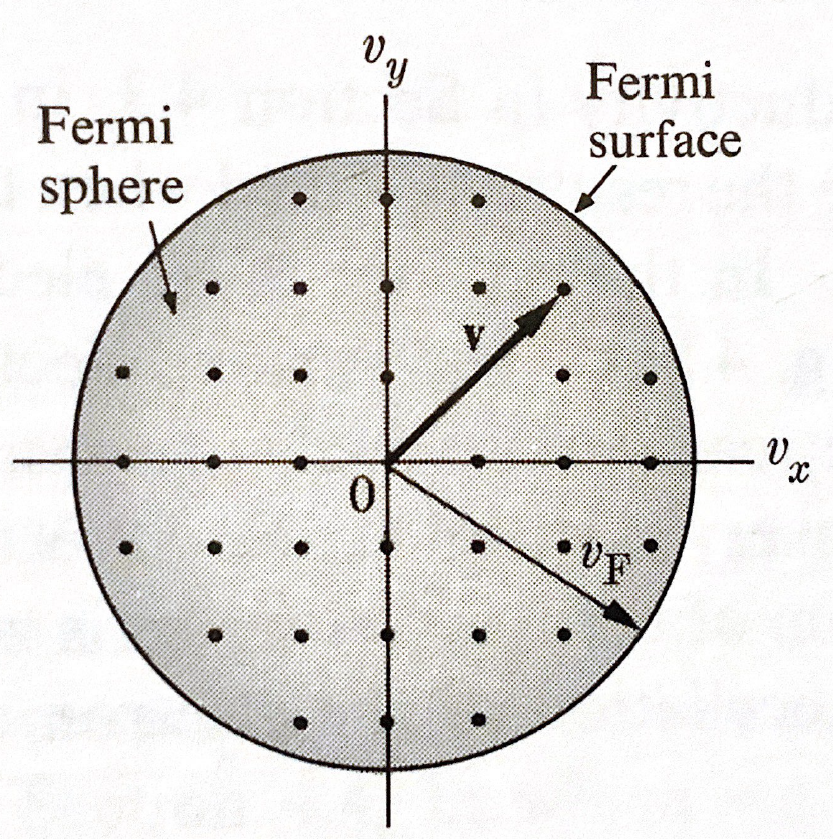
\includegraphics[width=0.4\linewidth]{Graphics/Chapter1/Fermi_Sphere.png}
    \caption{The Fermi surface and the Fermi sphere \cite[Elementary Solid State Physics p. 268]{elementary_SSP} }
    \label{}
\end{figure}

\subsubsection*{Cyclotron Frequency}

By applying a magnetic field to an metal, the electron inside are 
caused to move in a counterclockwise circular fashion. 
The frequency is called the cyclotron frequency.

\autoref{fig:Cyclotron_motion} shows this schematically. 

\begin{figure}[H]
    \centering
    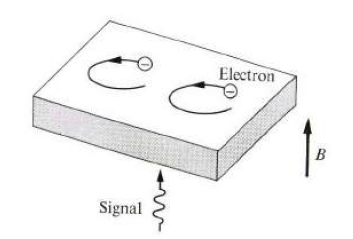
\includegraphics[width=0.4\linewidth]{Graphics/Chapter1/cyclotron_motion.png}
    \caption{Cyclotron Motion \cite[Elementary Solid State Physics p. 160]{elementary_SSP} }
    \label{fig:Cyclotron_motion}
\end{figure}

The motion of an electron in a magnetic field can be 
described by the following differential equation.

\begin{equation}
    -e (\vec{v} \times \vec{B}) =  m \frac{d\vec{v}}{dt}
\end{equation}

With the given information that $\vec{B} = B\vec{z}$.\\
The equation above lead to the following two 
equation.

$$-e v_y B = m \frac{d}{dt}v_x$$
$$e v_x B = m \frac{d}{dt}v_y$$

Which can be solved with the additional information $$k(0) = k_{0x}$$

$$\vec{k} = k_{0x} \cos(\left(\frac{eB}{m^*}t\right) \hat{x} +  k_{0y} \sin \left(\frac{eB}{m^*}t\right) \hat{y}$$

This leads to the Cyclotron frequency of:

$$\omega = \frac{eB}{m^*}$$

\subsubsection*{Plasma Resonanz}

In the range of the plasma frequency the metalic medium acts
like a nonabsorbing transparent dielectric.
In \autoref{fig:PlasmaFrequency} the reflection coefficient
of a metal in dependence of the angular frequency is shown. 
The plasma region is where the reflection coefficient equals 
zero.

\begin{figure}[H]
    \centering
    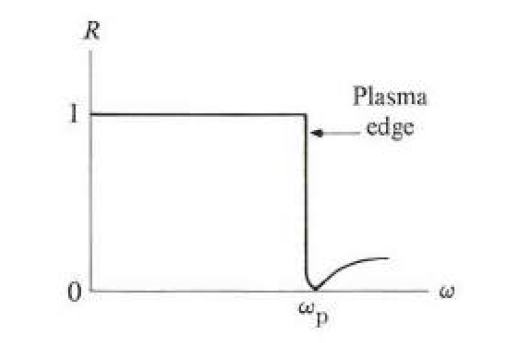
\includegraphics[width=0.6\linewidth]{Graphics/Chapter1/PlasmaFrequency.png}
    \caption{The plasma reflection edge.
    \cite[Elementary Solid State Physics p. 166]{elementary_SSP} }
    \label{fig:PlasmaFrequency}
\end{figure}

The plasma frequency can be calculated as:

\begin{equation}
    w_P^2 = \frac{Ne^2}{\epsilon_L m^*} \Rightarrow w_P = \sqrt{\frac{Ne^2}{\epsilon_L m^*}}
\end{equation}

With the parameter given $m^*=m_0$ and $\epsilon_L = \epsilon_0$:

$$w_P = 1.364 \cdot 10^{16} \frac{1}{s}$$

which corresponds to an energy of 

$$E_P = \hbar \omega = 1.439\cdot 10^{-23}J = 8.978eV$$